\documentclass{article}

\usepackage{xcolor}
\usepackage[margin=0.5in]{geometry} 
\usepackage{graphicx}

\graphicspath{{images/}}

\begin{document}

\newpage
\newgeometry{margin=1.5in}
\section*{Abstract}   % titolo temporaneo da modificare
In today's rapidly evolving business landscape, the importance of advanced technological tools becomes increasingly evident. The current market is characterized by swift and unpredictable changes, fueled by a myriad of factors such as technological advancement and the complex global geopolitical landscape. In this already intricate scenario, economic fluctuations and the growing expectations of consumers demand significant efforts from companies to remain competitive 
and meet the evolving needs of the market. All things considered, many uncertainties arise:

% NON E' UNA LISTA! -> mettere una lista sarebbe un errore (e' un flusso di domande, NON un elenco comprensivo!)
% sebbene quindi sbagliato penso pero' sia graficamente piu' piacevole, faro' la lista comunque
\begin{itemize}
    \item How will the market \textit{change} as these models become more efficient and effective?
    \item What \textit{must} companies do to remain competitive in the evolving market?
    \item What opportunities exist today for companies to \textit{harness} these technologies?
\end{itemize}
These were the uncertainties and presumptions of the present-day world.\\
% vvvvv riga vuota per enfatizzare l'ultima frase
\\
What follows is our response.
\\
\\
\\
\\
\\

\section*{MindMerge}
A web application focused on \textit{optimizing workflow}. The app allows users to create work schedules and tasks to assist businesses in dividing workloads. The flagship feature is the system - integrated with modern language models - that provides \textbf{fully automated reports} on personnel productivity, based on notes and comments provided by employees themselves in an easy and flexible manner.
\pagebreak
\restoregeometry

\section{Domain, Objectives}
Regarding the application domain, we have chosen Business Productivity for our project. Our decision was influenced by several factors. Certainly, the growing trend of public interest in AI has been a determining factor. The related market opportunities are promising, and B2B has historically always been promising. While our limited and relatively inexperienced team has certainly prevented us from implementing advanced features for our software, it has not impacted the choice of the system to develop.

\begin{enumerate}
\item \textbf{Enhanced Workflow Management}: Improve workflow management through detailed reports, easily obtainable through AI implemented within the software.
\item \textbf{Workload Optimization}: Optimize team members' workload by providing a real-time overview of current tasks and deadlines.
\item \textbf{Deadline Compliance Support}: Support adherence to deadlines through constant and real-time monitoring of tasks.
\item \textbf{Project Priority Management}: Effectively manage internal project priorities through a clear hierarchy of tasks to be completed.
\item \textbf{Communication Enhancement}: Improve communication and collaboration among employees by providing easy access to information for managers and colleagues.
\item \textbf{Scalability and Adaptability}: Ensure software scalability for projects of any size through a hierarchical structure of tasks and subtasks.
\item \textbf{Immediate Task Scheduling}: Schedule tasks immediately to reduce time spent in meetings, in an intuitive and practical manner.
\item \textbf{Employee Efficiency Evaluation}: Evaluate employee efficiency to optimize human resource utilization, eliminating the need for paper reports and individual interviews.
\end{enumerate}

\section{SWAT Analysis}
\subsection{Quick recap}
The development of software must incorporate a comprehensive evaluation of the economic environment in which it will operate.
Within this framework, the SWOT analysis emerges as a vital instrument for gaining a profound understanding of the surrounding landscape, enabling the formulation of a cohesive strategy to tackle challenges and leverage opportunities.

\begin{figure}[h]
  \centering
  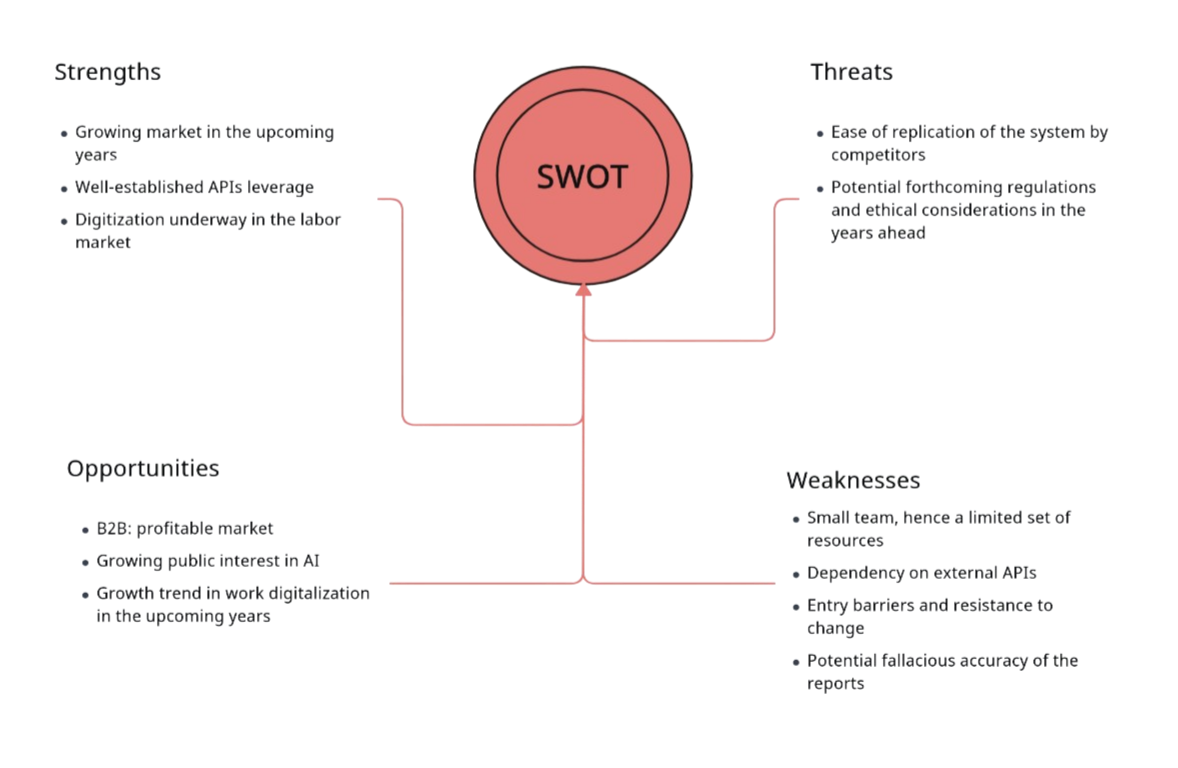
\includegraphics[width=0.95\textwidth]{swat_cropped.png}
  \caption{\small SWOT Analysis Diagram: visual representation of the Strengths, Weaknesses, Opportunities, and Threats associated with our software project}
\end{figure}

Here's a brief summary of the points outlined.
\begin{enumerate}
    \item \textbf{Strenghts}:\\
Predictions indicate that the LLM market is expected to grow by around \textbf{36\%} by 2030\footnote{source: grandviewresearch.com}. Having reliable and established APIs is a big plus as they offer more flexibility and are easy to incorporate. The ongoing shift towards digitalization in the job market provides opportunities for innovation and improving how companies manage their human resources.
    \item \textbf{Weaknesses}:
Moving on to weaknesses, our project has a few. Firstly, our team is small both in terms of finances and people. Depending too heavily on external APIs, even if they're reliable, is risky because our system relies heavily on them. Marketing our product and breaking into the market, which is competitive and growing, could be challenging. Resistance to change from employees at client companies is another hurdle. Lastly, ensuring the reliability of our reports and avoiding mistakes is crucial; if reports are inaccurate, it affects the usefulness and saleability of our product.
    \item \textbf{Opportuinities}:
The business-to-business (\textit{B2B}) market has always been profitable, as the buyer pool is to be found among market intermediaries rather than consumers. Furthermore, it's estimated to grow by \textbf{19\%} by 2031\footnote{source: straitsresearch.com}. LLMs are becoming more recognized in the public eye, which can work in our favor. Plus, ongoing trends in digitalization and innovation in our sector offer good opportunities.
    \item \textbf{Threats}:
Our project faces some potential risks. Firstly, there's the chance that competitors could easily copy our idea in the near future. Additionally, \textbf{future regulations} on AI could pose an economic threat. If restrictions are placed on LLMs, a significant part of our system would be affected. There's also the concern that ethical debates around work might become a problem, especially if there's widespread distrust or bans on AI in Western countries.
\end{enumerate}
\end{document}
